\begin{figure*}[ht]
    \centering
    \vspace{-3mm}
    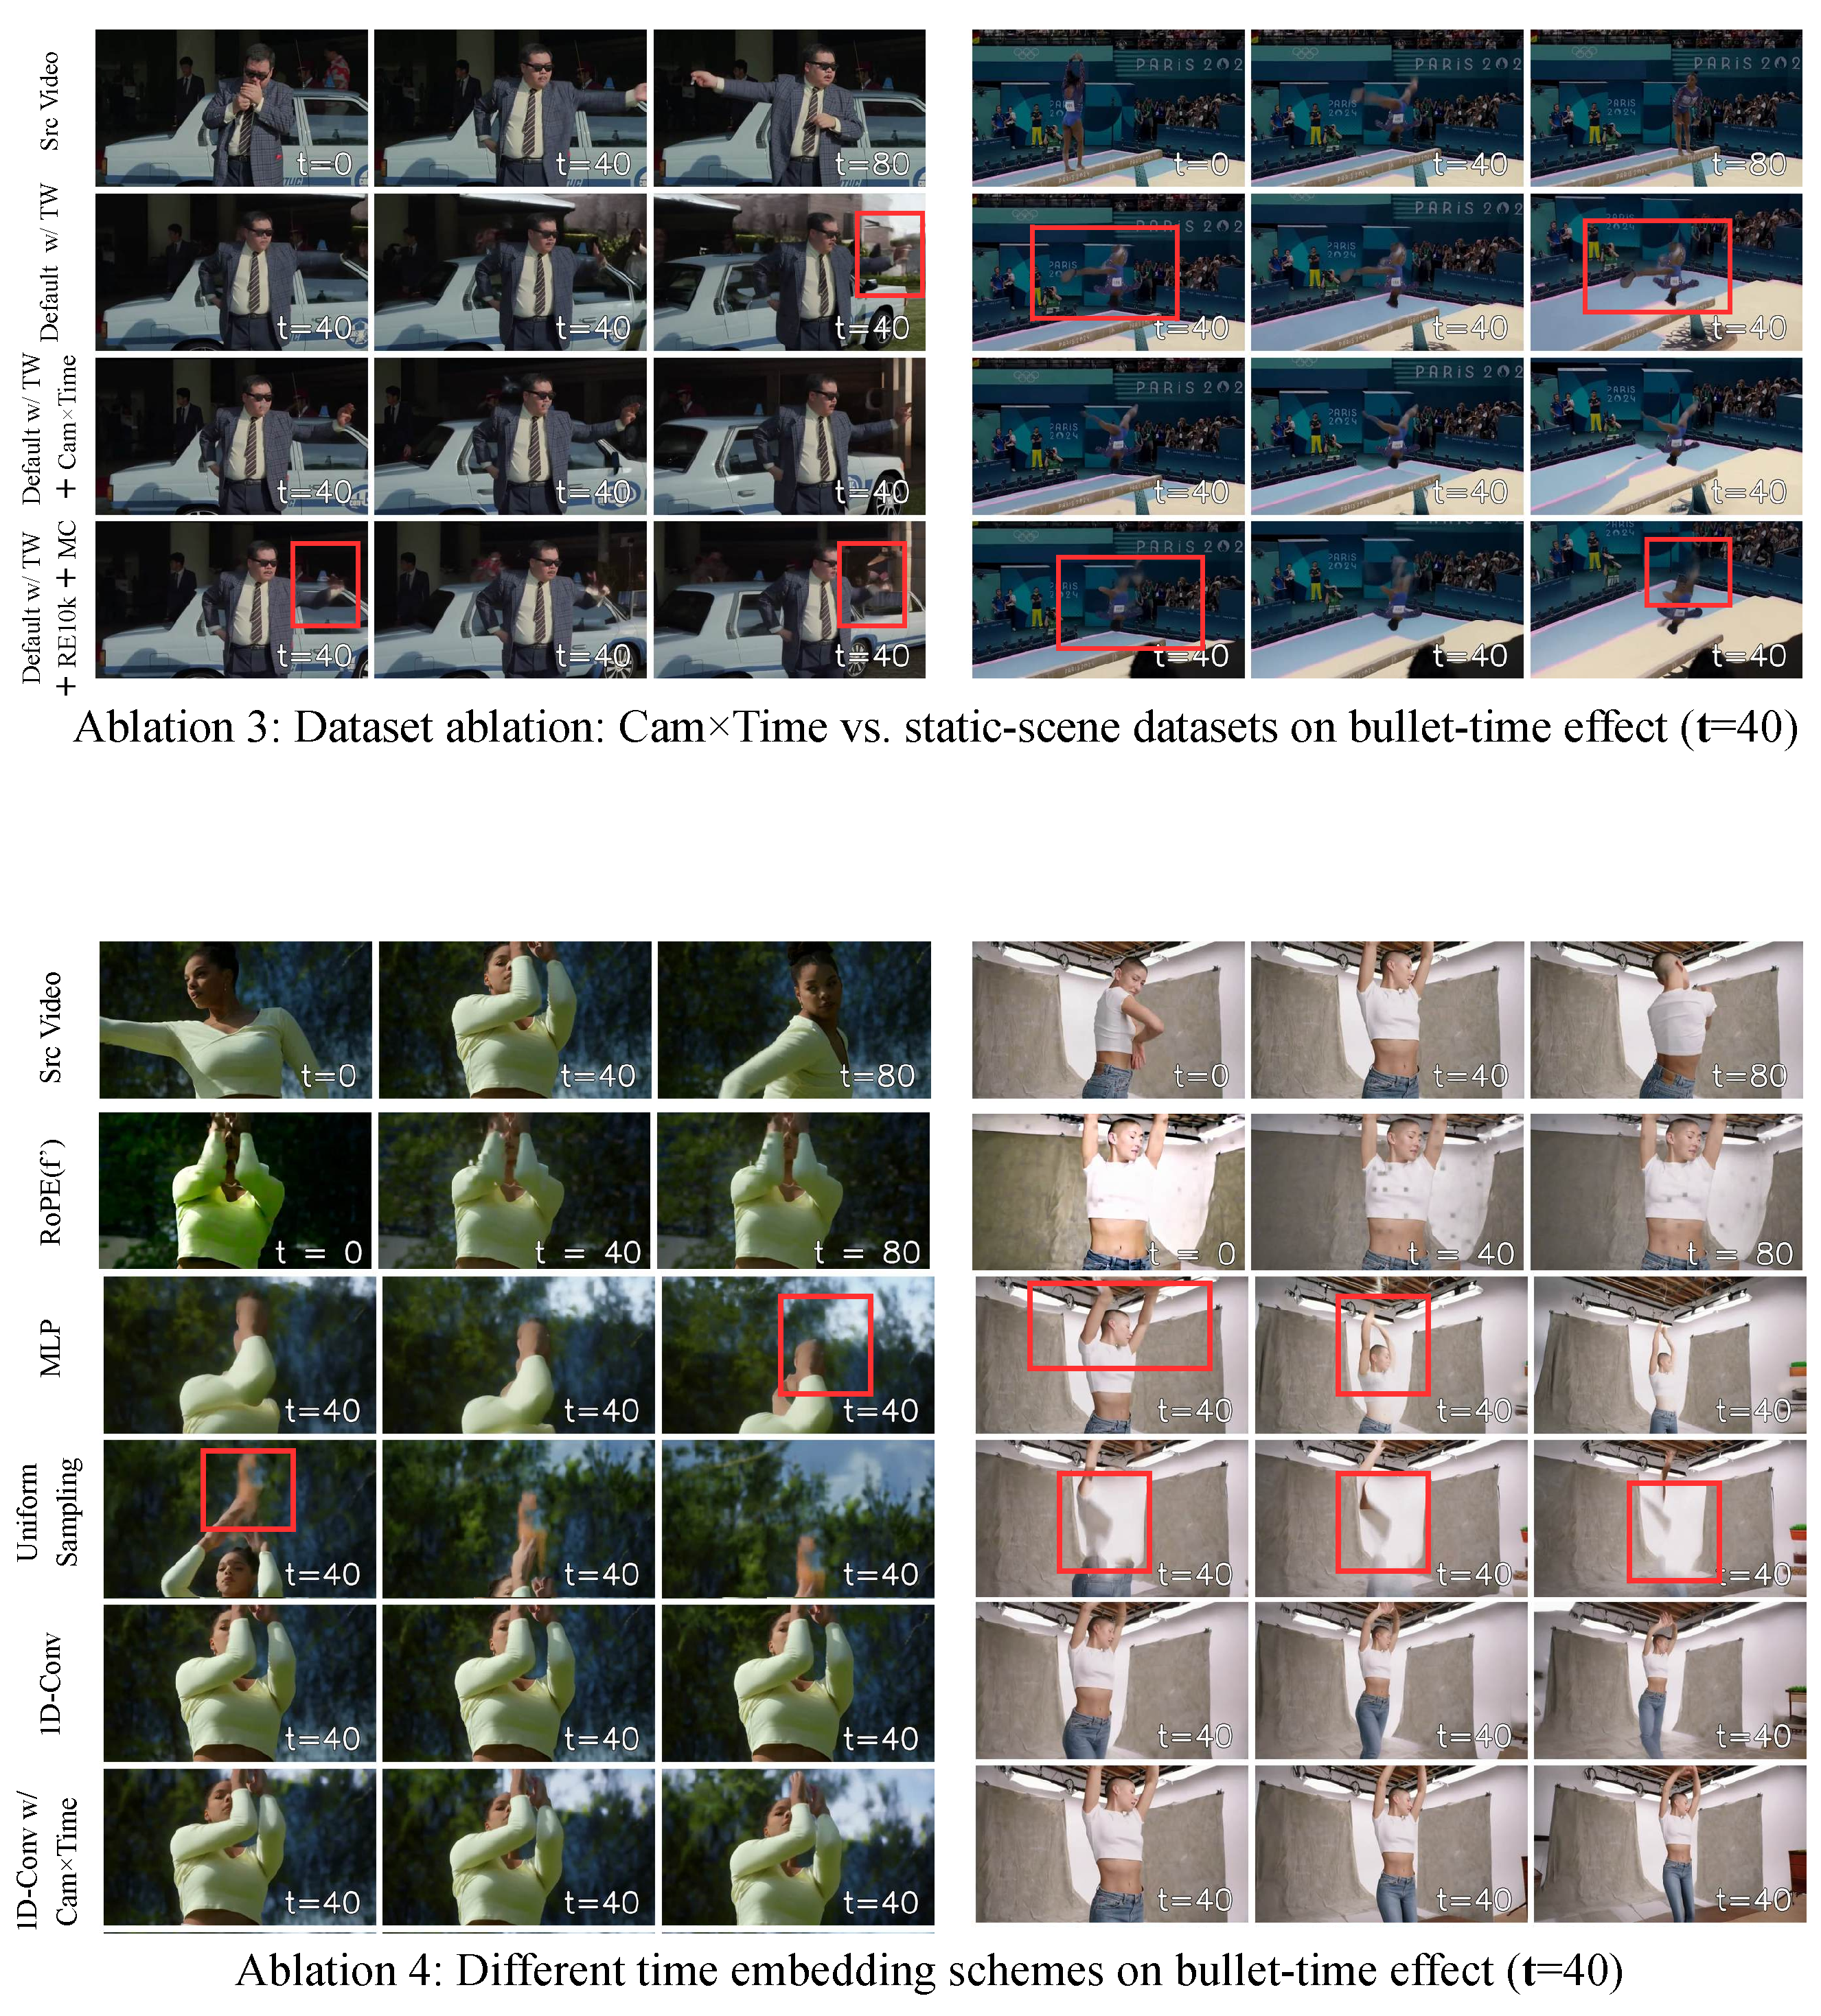
\includegraphics[width=\linewidth]{figures/src_files/ablation_3_4.pdf}
    
    \caption{
    \textbf{Ablation study.}
    (Top) We verify the efficacy of the proposed \nameDataset dataset. Considering \cite{Bai2025,bai2024syncammaster} as default datasets, we compare the impact of different datasets on the generated videos. One can clearly see artifacts in baselines without any extra data or augmented with static-scene data, whereas training additionally with \nameDataset leads to no artifacts, confirming the usefulness of our dataset.
    (Bottom) We compare several time-embedding strategies. The MLP fails to lock the temporal state (red boxes), while RoPE($f'$) correctly freezes the scene dynamics at $\animatime$=40 but unintentionally locks the camera motion too. Conditioning on the latent frame $f'$ (with uniform sampling) introduces noticeable artifacts. In contrast, the proposed 1D-Conv embedding allows \nameMethod to both freeze the scene dynamics at $\animatime$=40 and produce intended camera motion. Incorporating \nameDataset during training further improves performance.
    }
    \label{fig:ablation_3_4}
\end{figure*}
